%
% In the style of NAACL
%

\documentclass[11pt,letterpaper]{article}
\usepackage{naaclhlt2016}
\usepackage{times}
\usepackage{latexsym, amsmath, amssymb}
\usepackage{graphicx}
\usepackage{tabularx}
\usepackage{hyperref}

\naaclfinalcopy % Uncomment this line for the final submission
\def\naaclpaperid{***} %  Enter the naacl Paper ID here

% To expand the titlebox for more authors, uncomment
% below and set accordingly.
% \addtolength\titlebox{.5in}    

\newcommand\BibTeX{B{\sc ib}\TeX}


\title{Automated Identification and Extraction of Op-Ed Predictions Using Machine Learning\Thanks{This research was conducted under the guidance of Professor Chris Callison-Burch ({\tt ccb@cis.upenn.edu}), at the Computer Science Department of the University of Pennsylvania.}}
\date{April 28, 2016} 
% Author information can be set in various styles:
% For several authors from the same institution:
% \author{Author 1 \and ... \and Author n \\
%         Address line \\ ... \\ Address line}
% if the names do not fit well on one line use
%         Author 1 \\ {\bf Author 2} \\ ... \\ {\bf Author n} \\
% For authors from different institutions:
% \author{Author 1 \\ Address line \\  ... \\ Address line
%         \And  ... \And
%         Author n \\ Address line \\ ... \\ Address line}
% To start a seperate ``row'' of authors use \AND, as in
% \author{Author 1 \\ Address line \\  ... \\ Address line
%         \AND
%         Author 2 \\ Address line \\ ... \\ Address line \And
%         Author 3 \\ Address line \\ ... \\ Address line}
% If the title and author information does not fit in the area allocated,
% place \setlength\titlebox{<new height>} right after
% at the top, where <new height> can be something larger than 2.25in
\author{Lawrence Chan\\
		University of Pennsylvania\\
        Philadelphia, PA 19104\\
	    {\tt chanlaw@seas.upenn.edu}}

\begin{document}

\maketitle

\begin{abstract}
By scoring the predictive accuracy of political pundits, we can hold them accountable for bad predictions and reward better pundits. However, in order to score the predictive accuracy of pundits, their predictions must be first identified and extracted by hand, a laborious process that is a key limiting factor of this endeavor. In this paper we propose to use machine learning techniques to automate the identification and extraction process. We train various machine learning models and show that this approach has much promise. 
\end{abstract}

\section{Introduction}
The problem of poor predictive accuracy of the average pundits is well known amongst the forecasting literature. For example, a study of 284 experts and over 28,000 predictions, conducted by Philip Tetlock over a period of more than 20 years, found that experts performed barely better than chance \cite{Tetlock:05}. However, research has also shown a large degree of variation among the accuracy of forecasts, and so there is significant interest in tracking and scoring the accuracy of political pundits \cite{Tetlock:16}. Many even hope to make this a standard part of standard intellectual discourse, much like polling numbers are a necessary part of any discussion about election forecasts today. 

Nevertheless, this process of identifying and extracting predictions from the vast volume of editorial pieces published daily is a daunting task, even if we were to limit our attention to only a few of the most notable pundits. In this paper we propose using machine learning to partially resolve this problem. By trawling the writings of these pundits and returning excerpts containing their predictions, we can vastly reduce the amount of manpower needed for such a project. 
\subsection{What we mean by prediction}
In this context, a prediction is a statement that constrains our beliefs about the future. Predictions need not be certain - a statement that a certain future event is very likely or unlikely is also a prediction about the future, especially if the speaker assigns a probability estimate to the prediction. In order to be scored, predictions should be about events that we can verify objectively, at least in principle, a condition known as the "Clairavoyance Test" \cite{Tetlock:15}. Examples of sentences that we consider predictions and non-predictions are included in \textbf{Table \ref{predictions}}.
\begin{table}
\centering
 \begin{tabular}{| p{3.5cm} | p{3.5cm} |} 
 \hline
\textbf{Prediction} & \textbf{Non-prediction} \\
 \hline
\small{Trump is a long shot for the general election.} & \small{Trump is a con man and a crook.} \\
\hline
\small{Returning to the gold standard will cause a recession.}& \small{We should increase funding for our children's education.} \\
\hline
\small{Sanders will be a stronger general election candidate than Clinton.} & \small{Clinton's dominance was based on her lead among non-whites.} \\
 \hline
 \end{tabular}
 \caption{Examples of predictions and non-predictions}
 \label{predictions}
\end{table}

\section{Approach}
\label{approach}
For this project, we decided on the following three-step approach for training a classifier to recognize predictions:
\begin{enumerate}
\item\textbf{Webscraping and Data Cleaning} First, we used webscraping tools to acquire 207 articles from the New York Times Column of Paul Krugman, a nobel-prize winning economist and one of the most famous liberal pundits in America. We then cleaned the dataset and segmented it into 3882 sentences. 
\item \textbf{Crowdsourcing} We then used Crowdflower, a crowdsourcing website, to label the 3882 sentences as containing predictions or not containing predictions. 
\item \textbf{Machine Learning Classifier} Finally, we vectorized the sentences using a bag of words model, and then trained various machine learning models on this dataset, using a 80\% training, 10\% validation, and 10\% test set split. 
\end{enumerate}
More explanation for the rationale behind this three step approach is detailed in the next subsection, and more specifics about each of the three steps are available in each of their corresponding sections. A summary of the dataset is presented in table \ref{data}. The code and data used in this project is available online. \footnote{\href{https://github.com/chanlaw/prediction-extraction}{\texttt{github.com/chanlaw/prediction-extraction}}} 
\begin{table}
\centering
 \begin{tabular}{|c c c|} 
 \hline
\textbf{Articles} & \textbf{Sentences} & \textbf{Unique Words} \\
 \hline
207 & 3882 & 7621\\
 \hline
 \end{tabular}
 \caption{Summary of the dataset used. Articles were collected from Paul Krugman's New York Times Column.}
 \label{data}
\end{table}
\subsection{Rationale}
Our first attempt at classifying predictions was to use Hearst-like syntatical patterns to identify predictions \cite{Hearst:92}. However, despite creating combinations of rules, some with up to a dozen rules, we found that we could not beat the rule that always predicted that the given sentence contains no predictions on a hand-gathered test set of 150 sentences. This is in line with research showing the limitations of Hearst patterns in comparison to machine learning based models \cite{Snow:04}. As such, we abandoned this approach in favor of one using machine learning classifiers. 

Since no corpus of prediction-containing sentences currently exists, we decided to create our own dataset using webscraping and crowdsourcing. After considering various political pundits, we settled on Paul Krugman as a famous pundit who made significant more predictions than other pundits, averaging more than one per article. (For example, the Pulitzer-winning journalist Thomas Friedman makes almost no concrete predictions at all in his articles.) Because of the size of the dataset required to train a classifier, we decided to label the dataset using crowdsourcing. 

We explored segmenting the dataset using other methods - both in terms of longer excerpts (at paragraph level) and in terms of shorter excerpts (at the phrase level). Ultimately, we chose to segment the articles at the sentence-level, because this seemed like a good compromise between having sufficiently a large dataset and having enough information to identify predictions.
\section{Webscraping and Data Cleaning}
\label{sec:webscraping}
We used Python's \href{https://docs.python.org/2/library/urllib2.html}{\texttt{urllib2}} package and the \href{https://www.crummy.com/software/BeautifulSoup/}{\texttt{Beautiful Soup}} Python Library to extract the content from the first 55 pages of Paul Krugman's column, \href{http://krugman.blogs.nytimes.com/}{The Conscience of a Liberal}. We took advantage of the fact that the formatting of all New York Times columns is standardized; by extracting html items with the class "story-body-text", we were able to get the content of the articles without having to use an API to clean the scrapped html. A total of 207 articles were extracted (Krugman's weekly music sharing posts were ignored). We then used NLTK, a natural language processing package, to segment the articles into sentences. We obtained a total of 3882 sentences through this process. 
\section{Crowdsourcing}
\label{sec:crowdsourcing}

\begin{figure*}[t]
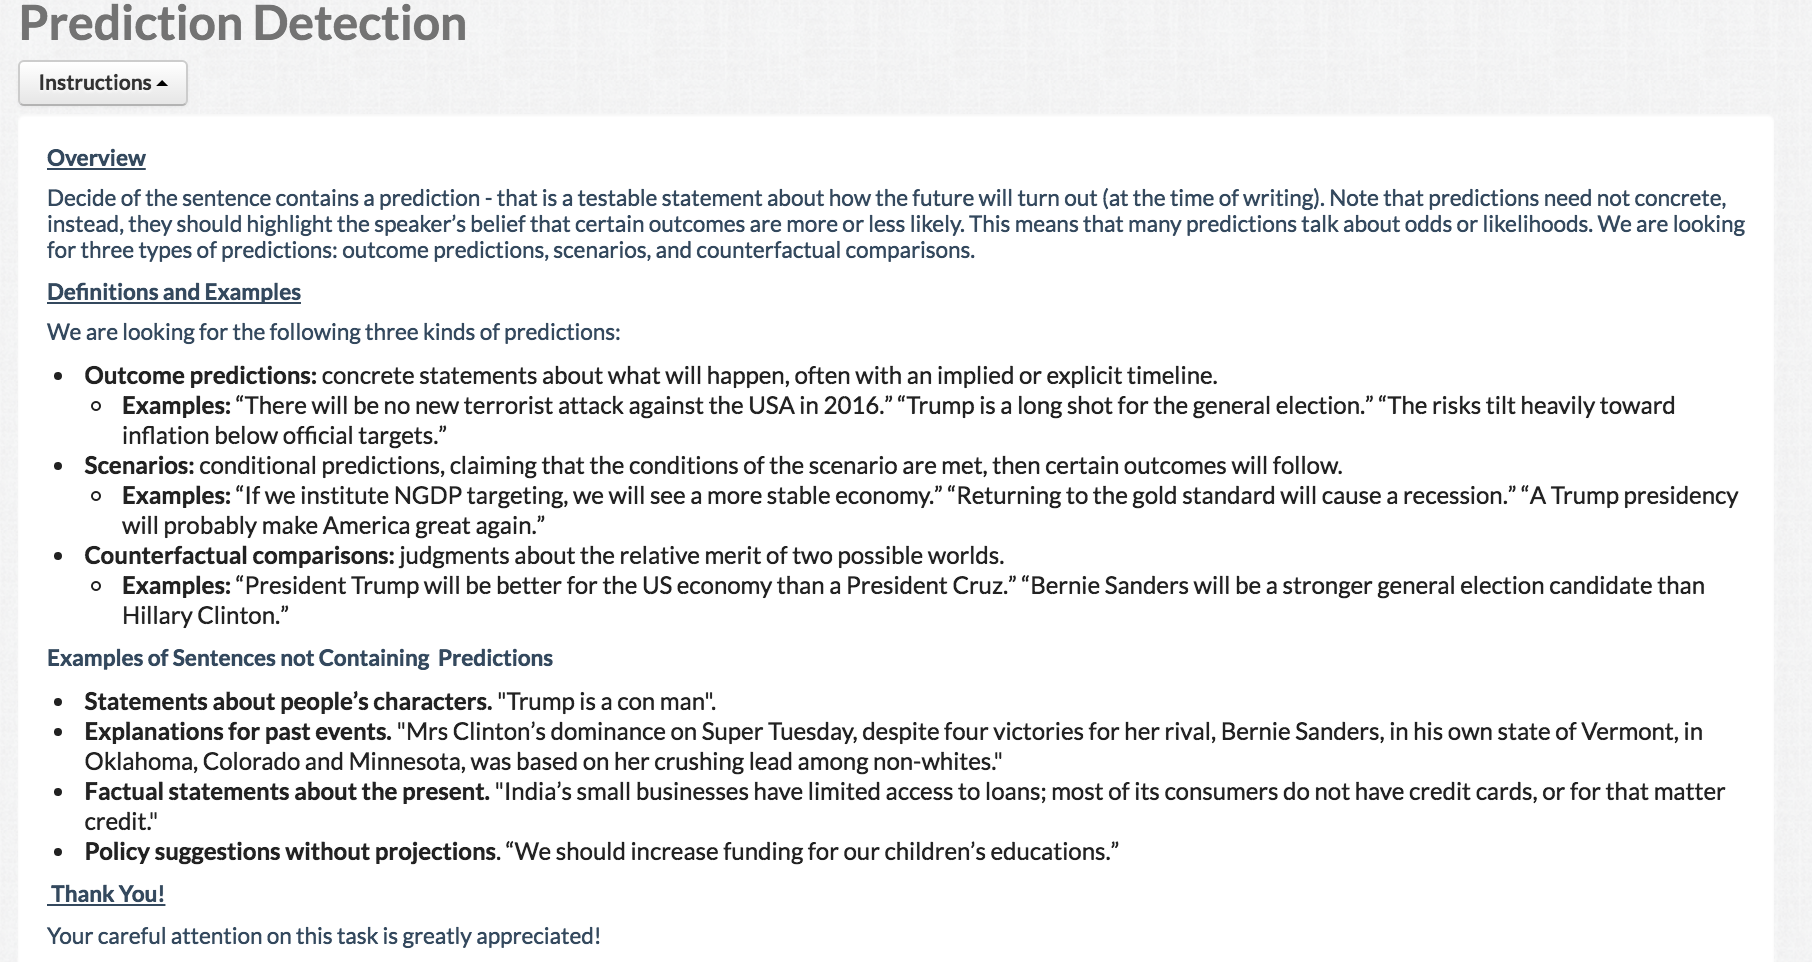
\includegraphics[width=\textwidth]{taskdescription.png}
\centering
\caption{Final task description given to contributors.}
\label{description}
\end{figure*}
After we obtained the dataset of segmented sentences, we used Crowdflower to label the sentences. Crowdflower was chosen at the suggestion of Professor Callison-Burch for its ease of use and its support for data validation by using test questions to filter out untrustworthy contributors. We paid contributors \$0.11 for every set of 8 sentences (7 to be labelled and 1 test). In order to guarantee accuracy, we had each sentence labelled by 3 different contributors, and took the majority opinion for each sentence. The total cost for all 3882 sentences, including the 20\% fee charged by Crowdflower and payments to individuals who failed the test questions, was \$250.95, or \$0.064 per sentence and \$1.21 per article. 

We used an iterative process to design the Crowdsourcing instructions for the task. We wrote three different sets of instructions and ran each of them through Crowdflower with a test set of 100 sentences. The contributor ratings for the three test runs are displayed in \textbf{Table \ref{ratings}}. We then used the best instruction set, which we display in \textbf{Figure \ref{description}}, to label the entire dataset. 

 In total the crowd identified 454 predictions in the 3882 sentences.  
\begin{table}
\centering
 \begin{tabular}{|l |c c |} 
 \hline
\textbf{ Attempt} & \textbf{Overall} & \textbf{Instructions}\\
 \hline
Test Run 1 & 3.4 & 3.6\\
Test Run 2 & 3.1 & 3.6\\
Test Run 3 & 4.2 &  4.3\\
Final Run & 4.2 & 4.3 \\
 \hline
 \end{tabular}
 \caption{Contributor ratings of labelling task (out of 5)}
 \label{ratings}
\end{table}


\begin{table*}[t]
\centering
 \begin{tabular}{|l |c  c  c |} 
 \hline
\textbf{Classifier} & \textbf{Accuracy} & \textbf{Recall} & \textbf{Precision}\\
 \hline
Logistic (50k Most Frequent Uni/Bi/Trigrams) & 0.911 & 0.358 & 0.755\\
Logistic (10k Most Frequent Uni/Bigrams) & 0.911 & 0.347 & 0.751 \\
SVM (RBF Kernel) & 0.911 & 0.382 & 0.708 \\
Logistic & 0.908 & 0.354 & 0.711\\
SVM (Linear Kernel) & 0.907 & 0.377 & 0.681\\
Random Forest (100 Trees) & 0.899 & 0.124 & 0.881 \\
Naive Bayes & 0.892 & 0.319 & 0.616\\
Random Forest (10 Trees) & 0.890 & 0.153 & 0.739 \\
Naive Bayes (50k Most Frequent Uni/Bi/Trigrams) & 0.890 & 0.163 & 0.704\\
Naive Bayes (10k Most Frequent Uni/Bigrams) & 0.886 & 0.179 & 0.674 \\
Majority Class Classifier & 0.883 & 0.00 & N/A \\
 \hline
 \end{tabular}
 \caption{Averaged test-set performance of classifiers, in declining order of accuracy. Except where otherwise noted, models were trained with a feature set consisting of the 1000 most common unigrams.}
 \label{accuracies}
\end{table*}
\section{Machine Learning Classifier}
\label{sec:mlclassifier}
After removing punctuation and capitalization, we segmented each sentence into words. We then vectorized the sentences using a bag of words (unigram) model of the most frequent 1000 words, from a dataset containing 7621 unique words. We also used two alternate vectorizations, one using the 10,000 most frequent unigrams and bigrams, and another using the 50,000 most frequent unigrams, bigrams, and trigrams. 

With this dataset, we turned trained four kinds of classifiers: regularized logistic regression, support vector machines (SVMs) with both RBF and linear kernels, random forests with 10 and 100 trees, and naive Bayes. 

For each classifier, we performed 20-fold cross validation. In each fold, we split the dataset into  80\% training, 10\% validation, and 10\% test set, fit the models on the training set and used the validation set to tune the regularization parameter. For our logistic regression and support vector classifiers, the regularization parameter was $C$, the inverse regularization strength, chosen over a grid between $0.01$ and $100$; for random forest, it was the max depth of the tree, which varied between 1 and 30; and for naive Bayes, it was the smoothing parameter $\alpha$, chosen over a grid between 0.1 and 100. We then recorded the performance of each classifier on the test set. Due to limitations on computing power, we were not able to train a support vector machine and random forest classifier on the unigram/bigram mix or the unigram/bigram/trigram mix.

\section{Results}
\label{results}
Our results are displayed in \textbf{Table \ref{accuracies}}. Overall, logistic regression over the uni/bi/trigram mix, logistic regression over the uni/bigram mix, and SVM using the RBF kernel did the best, with an average test-set accuracy of 0.911. Logistic regression on the unigram dataset and SVM using a linear kernel were in the second tier, with an average test-set accuracy of 0.908 and 0.907, respectively. This makes sense because both logistical regression including bigrams and SVMs using the RBF kernel can draw nonlinear boundaries around words, while logistic regression using only unigrams and Linear SVMs can only draw linear boundaries with respect to the words in the feature set. This is further supported by the most informative features for the models (displayed in \textbf{Table \ref{features}}). 

\begin{table}
\centering
 \begin{tabular}{|c | c|} 
 \hline
\textbf{Logistic (Uni/Bi/Trigram)} & \textbf{Logistic (Uni/Bigram)}  \\
 \hline
will & will\\
would & wont \\
going to & would \\
if & going to \\
wont & if\\
 \hline
 \hline
\textbf{Logistic (Unigram)} & \textbf{SVM (Linear Kernel)}  \\
 \hline
will & will\\
going & going\\
wont & wont\\
raise & raise\\
likely & unless\\
 \hline
 \end{tabular}
 \caption{Most informative features for linear classifiers}
 \label{features}
\end{table}

Note that random forest classifiers and naive Bayes performed very poorly on the dataset. The majority class classifier, which always predicts "no" on every sentence, performs almost as good as these classifiers. This is in line with the properties of the classifiers - while support vector machines and logistic regression are often used for text classification, random forest classifiers and naive Bayes do much more poorly in this domain due to the assumptions they make about the data \cite{Hastie:13}.

\begin{table*}
\centering
 \begin{tabular}{| p{6.5cm} | p{6.5cm} |} 
 \hline
\textbf{False Positives} & \textbf{False Negatives}  \\
 \hline
If Britain does leave the EU, and escapes the grip of the Eurocrats, who will it be empowering instead? & Falling oil leads to falling inflation expectations, and since interest rates can't fall, real rates go up, hurting recovery.\\
\hline
But what really amazes me about the latest set of stories is the promise that Ryan will finally deliver the Republican Obamacare alternative that his colleagues in Congress have somehow failed to produce after all these years. & True socialized medicine — an American NHS — would be feasible economically; so would single-payer, in the form of Medicare for all.\\
 \hline
 \end{tabular}
 \caption{Representative errors on new dataset}
 \label{errors}
\end{table*}
Using our best performing logistic regression model, we acquired and labelled a new dataset of 272 sentences from Paul Krugman's column. 11 sentences were labelled as predictions. The labelled dataset was then hand-graded for accuracy, and we identified 3 false positives and 11 false negatives, meaning our model had recall 0.42 and precision 0.727. We present representative errors in \textbf{Table \ref{errors}}. All three of the false positives have phrases that seem very much like real predictions made by the author, but were either questions asked by the author or commentary on predictions made by other. The false negatives were more varied; some are predictions not including words such as "will" or "would", while others were simply misclassified for no easily identified reason.  

\section{Discussion}
\label{discussion}
We believe that the results above demonstrate that this approach is a viable one. By using webscraping and machine learning techniques, we can significant reduce the amount of time used in labeling extracting predictions, saving manpower for other uses. In particular, the high precision of our classifiers could greatly reduce the amount of text a researcher needs to read to identify a prediction.

However, we believe that there exists significant room for improvement.  Even an accuracy rate of 0.911, the best we could achieve, is not particularly impressive, given that the majority class classifier achieves an accuracy of 0.883. The classifiers we trained were all relatively low recall - the highest recall we achieved was less than 0.4. We have identified three ways to improve this result. 

First, we can improve the dataset of labelled sentences, both in terms of quantity and quality. Because the cost of crowdsourcing is relatively low - another 10000 sentences will cost less than \$700 - this seems like a simple next step. In addition, the crowdsourced labels could probably be higher quality - the average agreement between crowd-sourced labels and hand-labelled dataset is around 95\%. We can do this by either paying more and recruiting higher quality crowdworkers, or by recruiting Penn students to label the data. 

Second, we can try to improve the way our classifiers are trained. For example, since the current generation of classifiers all demonstrate low recall, boosting could be used to improve their performance on false negative examples. A third and final improvement would be to find a better way of vectorizing the data, relative to the current bag-of-words type models. For example, we could try Google's \href{https://code.google.com/archive/p/word2vec/}{Word2Vec} or other low-dimensional word-level embeddings, or even use a sentence-level representation that preserves the order, as done by Le and Mikolov \cite{Le:14}. 


\bibliography{bibliography}
\bibliographystyle{naaclhlt2016}


\end{document}